\section{Kết quả và Phân tích so sánh}
Phần này trình bày kết quả đánh giá thực nghiệm của phương pháp đề xuất trên bộ dữ liệu CICIDS2017.

\subsection{Đánh giá tổng thể hiệu năng và độ trễ suy luận}
Bảng~\ref{tab:overall_results} so sánh hiệu năng và chi phí tài nguyên của tất cả các mô hình trên tập kiểm tra độc lập (giữ nguyên tỷ lệ mất cân bằng ban đầu).

\begin{table}[htbp]
\centering
\caption{So sánh hiệu năng, độ trễ và dung lượng bộ nhớ của các mô hình}
\label{tab:overall_results}
\footnotesize
\begin{tabular}{@{}l@{\hspace{3.5pt}}c@{\hspace{3.5pt}}c@{\hspace{3.5pt}}c@{\hspace{3.5pt}}c@{\hspace{3.5pt}}c@{}}
\toprule
\textbf{Mô hình} & \textbf{Acc.} & \textbf{F1} & \textbf{AUC} & \textbf{Trễ (ms/1k)} & \textbf{Size (MB)} \\
\midrule
XGBoost          & 0,9986 & 0,9960 & 0,9999 & -- & --  \\
LightGBM         & 0,9987 & 0,9961 & 0,9999 & -- & --  \\
Random Forest    & 0,9985 & 0,9957 & 0,9999 & -- & -- \\
\midrule
\textbf{Stacking (GV)} & \textbf{0,9987} & \textbf{0,9963} & \textbf{0,9999} & 60189,94 & 22,50 \\
\textbf{Học viên (ĐX)} & \textbf{0,9948} & \textbf{0,9845} & \textbf{0,9992} & \textbf{163,62} & \textbf{0,0128} \\
\bottomrule
\end{tabular}
\end{table}

\begin{table}[htbp]
\centering
\caption{So sánh với các công trình gần đây trên CICIDS2017}
\label{tab:literature_comparison}
\footnotesize
\begin{tabularx}{\columnwidth}{@{}p{2.3cm}Xcc@{}}
\toprule
\textbf{Nghiên cứu} & \textbf{Phương pháp} & \textbf{Acc. (\%)} & \textbf{F1 (\%)} \\
\midrule
Amara et al. (2025)~\cite{amara2025stacked}     & CNN+TCN+LSTM Ens.     & 99,99 & 100,0 \\
Nguyen et al. (2024)~\cite{nguyen2024apelid}    & Augmented WGAN + Ens. & 99,78 & --    \\
Ding et al. (2024)~\cite{ding2024tmg}           & TMG-GAN + DNN         & 99,81 & 99,72 \\
Khan et al. (2024)~\cite{khan2024balanced}       & SMOTE-Tomek + DT      & 99,96 & --    \\
Hu et al. (2024)~\cite{hu2024improved}          & Hybrid Attention      & 99,79 & --    \\
Ji (2025)~\cite{ji2025hybrid}                   & GRU-ResCBANet         & 99,83 & --    \\
Sarhan et al. (2022)~\cite{sarhan2022towards}   & ML Baseline (TII)     & 99,70 & 99,20 \\
\midrule
\textbf{Stacking Giáo viên}                     & \textbf{Hybrid Ensemble} & \textbf{99,87} & \textbf{99,63} \\
\textbf{Cây Học viên (Chưng cất)}               & \textbf{Lightweight DT}  & \textbf{99,48} & \textbf{98,45} \\
\bottomrule
\end{tabularx}
\end{table}

Mô hình Stacking Giáo viên đạt hiệu năng cực cao trên tất cả chỉ số (F1 0,9963), chứng minh hiệu quả của việc kết hợp boosting và bagging. Đặc biệt, mô hình cây quyết định Học viên sau chưng cất vẫn duy trì hiệu năng tuyệt vời (Acc 0,9948; F1 0,9845), tiệm cận mô hình Giáo viên phức tạp. Tuy nhiên, về mặt triển khai, mô hình Học viên mang lại hiệu quả vượt trội: tốc độ suy luận tăng khoảng \textbf{368 lần} (độ trễ giảm từ 60189,94 ms xuống còn 163,62 ms cho mỗi 1.000 mẫu) và kích thước mô hình được nén tới \textbf{1.758 lần} (từ 22,50 MB xuống còn 0,0128 MB). Kết quả này khẳng định tính khả thi của mô hình Học viên chưng cất khi triển khai tại biên thời gian thực.

\subsection{Đường cong AUC-ROC và AUC-PR}
Hình~\ref{fig:roc_pr} thể hiện đường cong ROC và PR của các mô hình. AUC-PR đặc biệt có ý nghĩa đối với dữ liệu mất cân bằng nghiêm trọng vì nó phản ánh chính xác chất lượng phát hiện trên các lớp tấn công thiểu số. Mô hình Stacking Giáo viên đạt AUC-PR là 0,9999, và cây quyết định Học viên sau chưng cất vẫn giữ mức AUC-PR rất cao (0,9992), khẳng định tính ổn định vượt trội khi nhận diện tấn công hiếm.

\begin{figure*}[htbp]
\centering
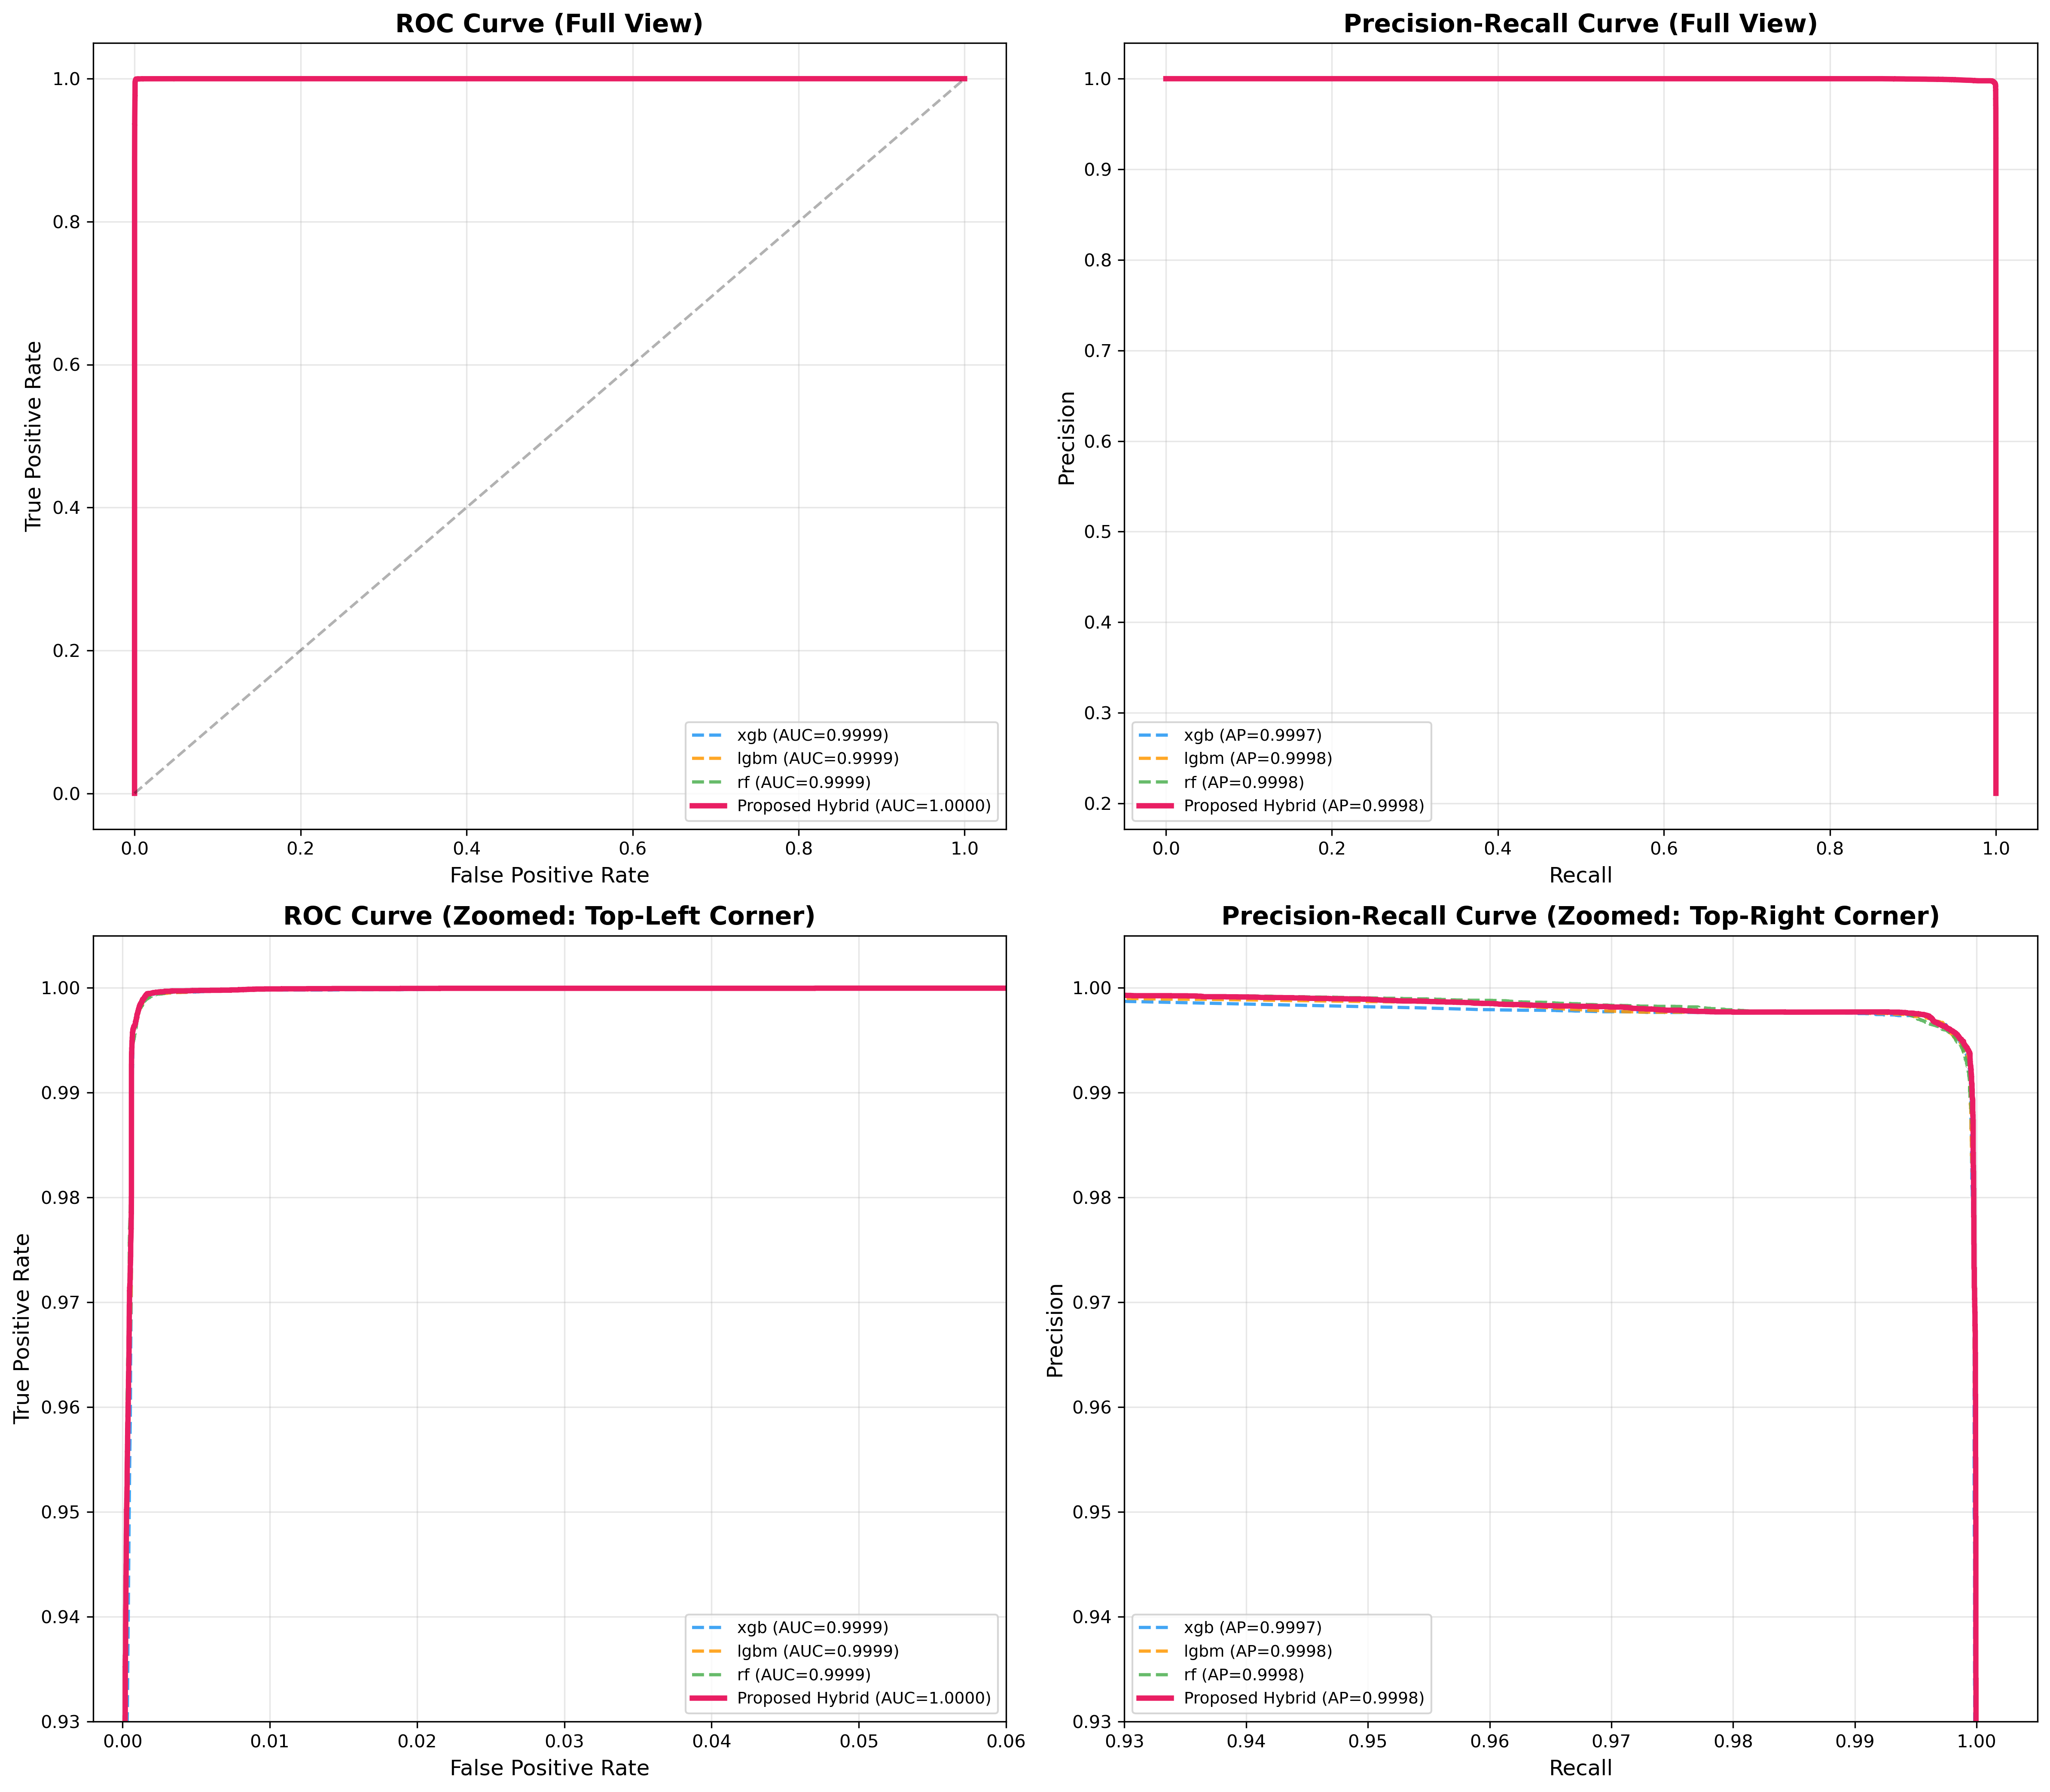
\includegraphics[width=\textwidth]{figures/roc_pr_curves.png}
\caption{Đường cong ROC và Precision-Recall của các mô hình (hiển thị toàn cảnh và góc phóng to).}
\label{fig:roc_pr}
\end{figure*}

\subsection{Ma trận nhầm lẫn và giảm thiểu cảnh báo giả}
Trong các triển khai phát hiện xâm nhập thực tế, tỷ lệ dương tính giả (FPR) cao gây ra hiện tượng quá tải cảnh báo cho các chuyên gia giám sát. Ma trận nhầm lẫn trên Hình~\ref{fig:cm} thể hiện số lượng mẫu phân loại chính xác của các mô hình. Sự kết hợp giữa chiến lược lấy mẫu cân bằng ENN và bộ phân loại meta stacking giúp mô hình đề xuất tối ưu hóa ranh giới phân lớp, giúp giảm thiểu tối đa các cảnh báo giả trong khi vẫn bảo đảm tỷ lệ phát hiện cao cho các mẫu tấn công hiếm.

\begin{figure*}[htbp]
\centering
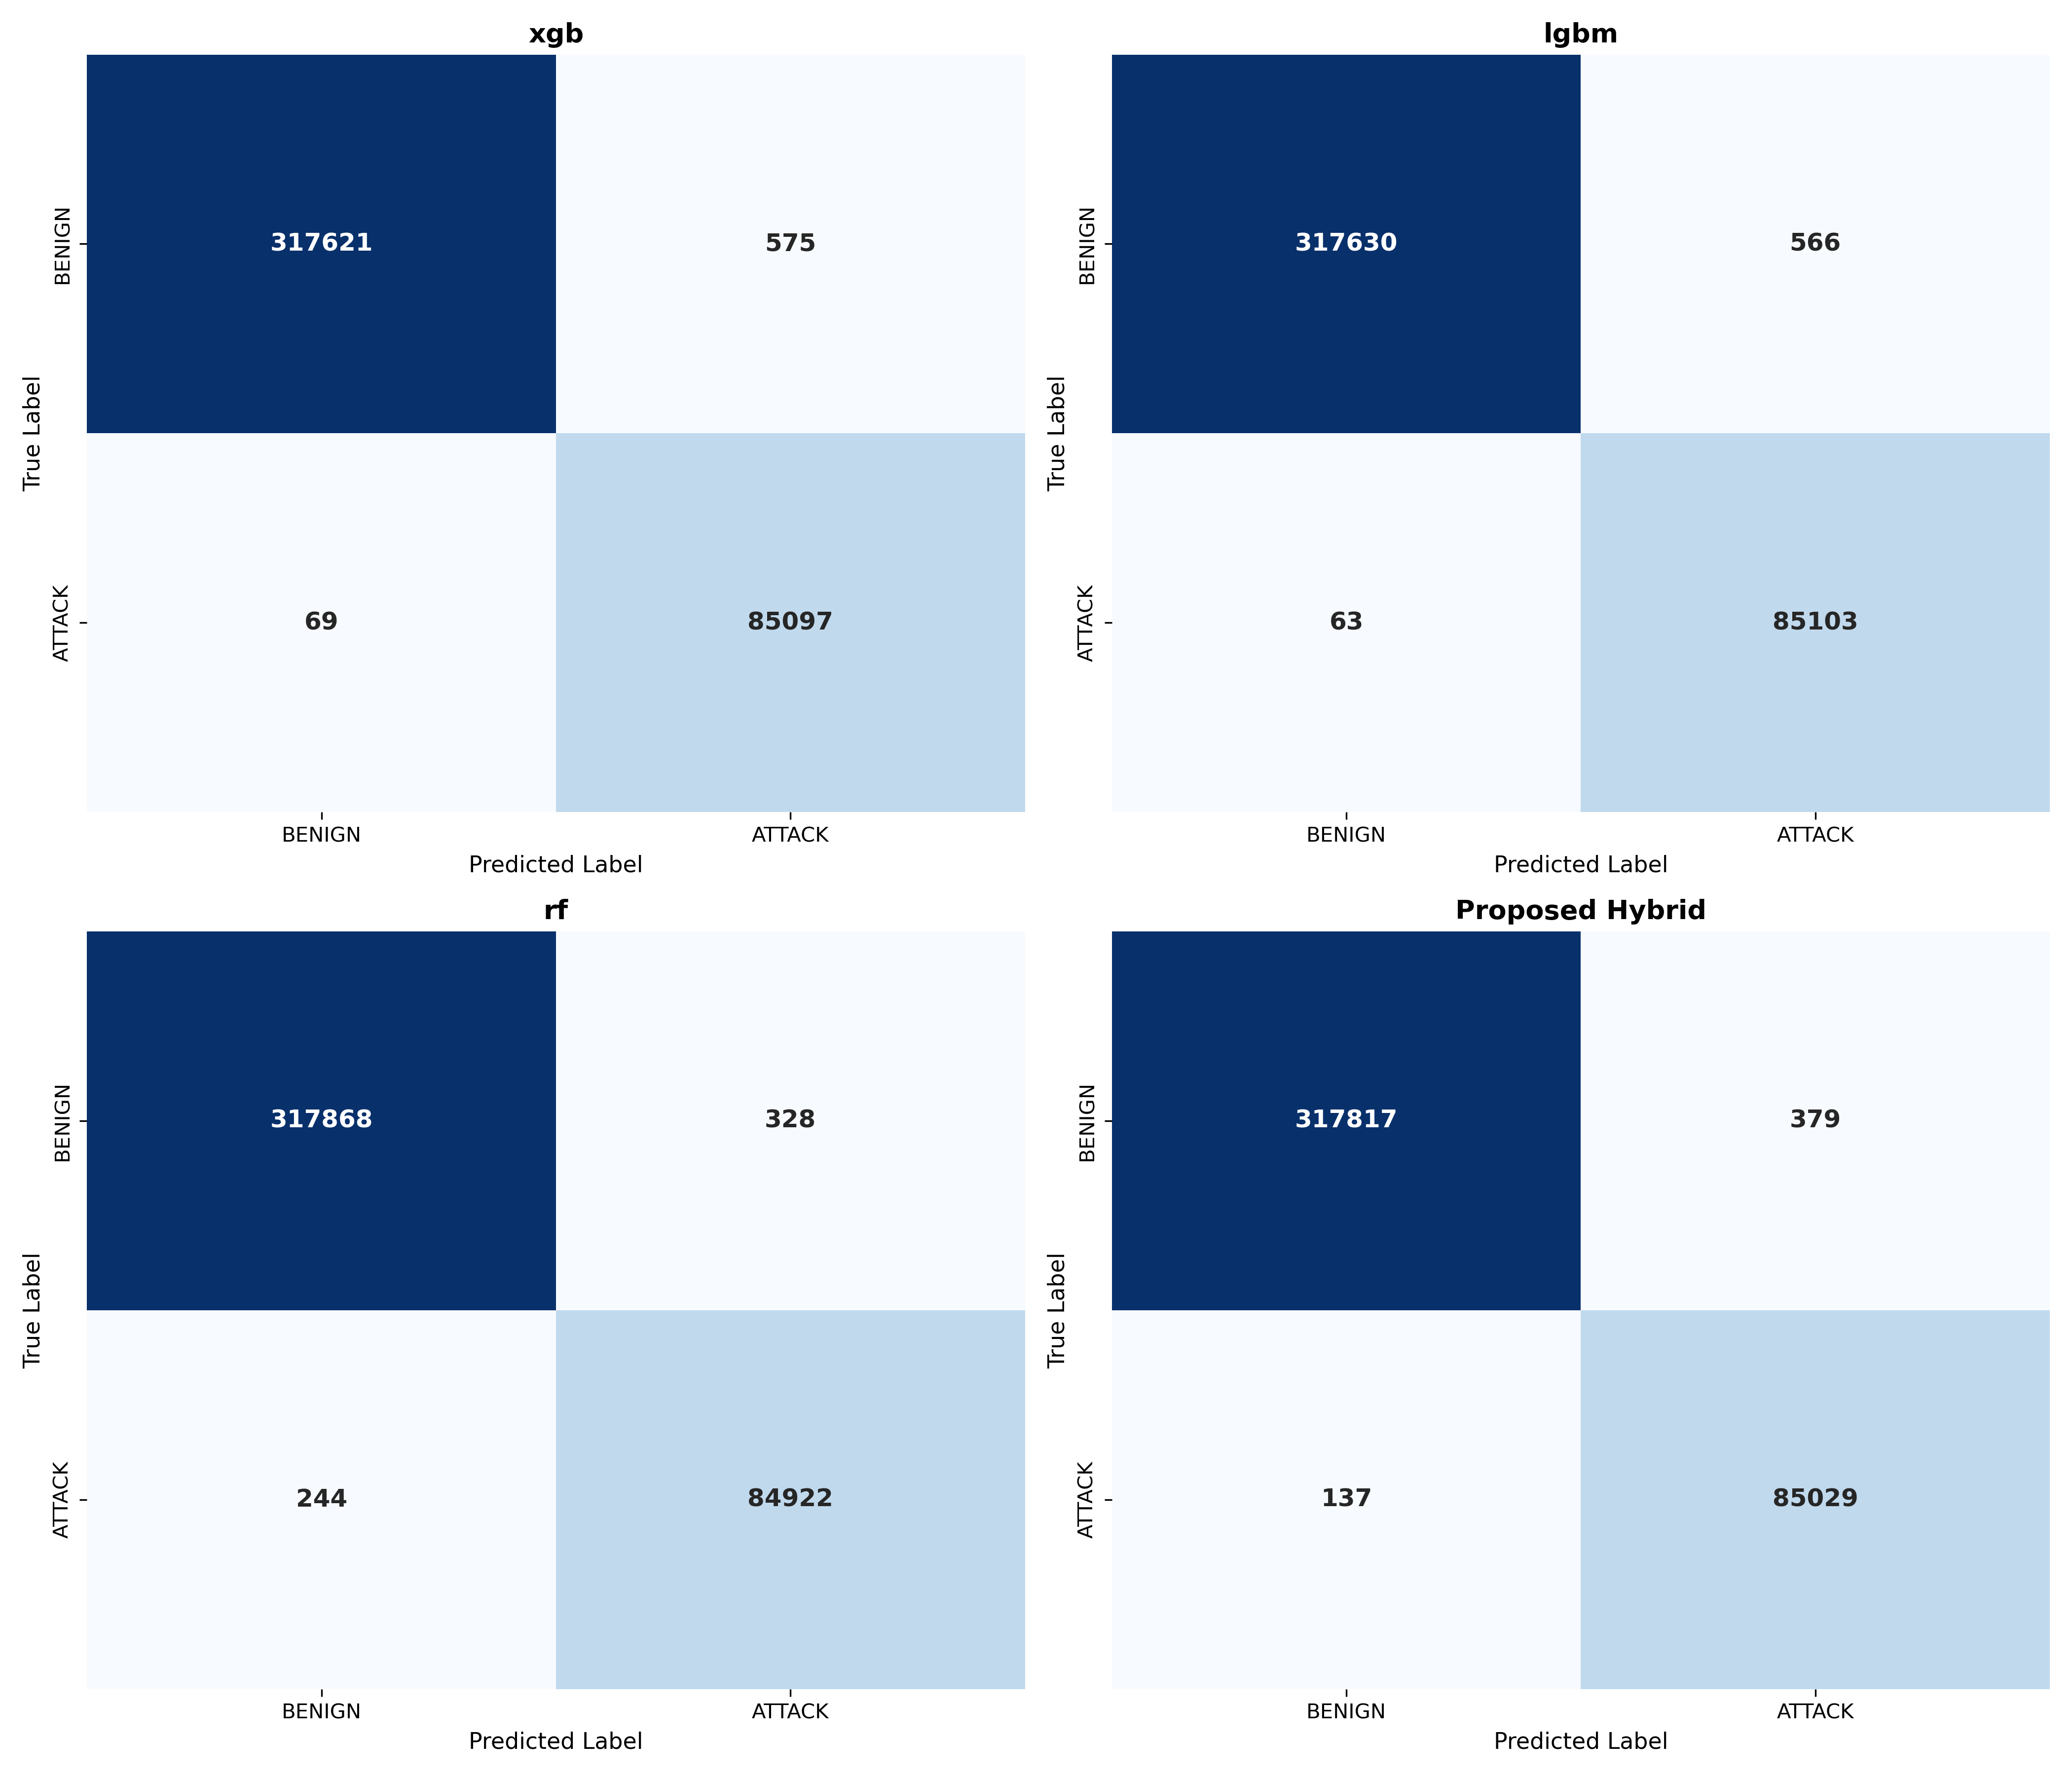
\includegraphics[width=\textwidth]{figures/confusion_matrices.png}
\caption{Ma trận nhầm lẫn so sánh các mô hình đơn lẻ và mô hình Stacking kết hợp Giáo viên.}
\label{fig:cm}
\end{figure*}

\subsection{Thử nghiệm bóc tách (Ablation Study)}
Chúng tôi thực hiện đánh giá để đo lường đóng góp của từng thành phần. Kết quả cho thấy: (1) Sử dụng ENN giúp giảm tỷ lệ dương tính giả (FPR) xuống mức rất thấp (0,0015), bảo vệ ranh giới lớp thiểu số; (2) Mô hình Stacking đạt kết quả tốt hơn cơ chế Soft Voting trung bình đơn giản nhờ việc tối ưu hóa trọng số của bộ phân loại meta; (3) Việc tích hợp thêm Random Forest cùng các mô hình boosting giúp gia tăng tính đa dạng và tăng độ chính xác tổng thể.

\subsection{So sánh với các nghiên cứu gần đây}
Bảng~\ref{tab:literature_comparison} đối chiếu hiệu năng mô hình đề xuất với các nghiên cứu NIDS công bố giai đoạn 2024--2026 trên tập dữ liệu CICIDS2017.

Giải pháp đề xuất đạt hiệu năng cạnh tranh so với các nghiên cứu hiện đại. Dù một số mô hình deep learning phức tạp đạt kết quả cao hơn một chút, chúng có chi phí tính toán rất lớn và không thể chạy thời gian thực tại biên. Trong khi đó, mô hình cây Học viên gọn nhẹ của chúng tôi có kích thước siêu nhỏ (0,0128 MB) và tốc độ phản hồi cực nhanh (163,62 ms/1k mẫu), tạo nên sự cân bằng tối ưu giữa hiệu năng và khả năng triển khai thực tế.

